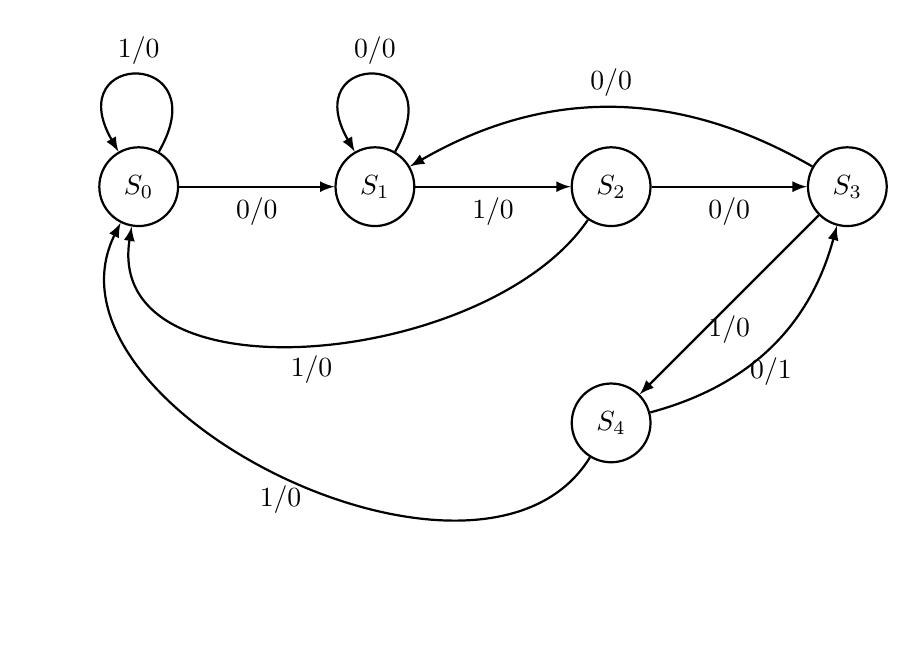
\begin{tikzpicture}[-latex ,node distance=3cm and 1cm,thick,state/.style={circle ,draw, minimum width =1cm}]
  \node[state] (S0) {$S_0$};
  \node[state] (S1) [right of=S0] {$S_1$};
  \node[state] (S2) [right of=S1] {$S_2$};
  \node[state] (S3) [right of=S2] {$S_3$};
  \node[state] (S4) [below of=S2] {$S_4$};

\path (S0) edge [loop above ,out=60, in=120, distance=1.5cm] node {1/0} (S0)
      (S2) edge [bend left , out=55, in=80] node [below=0.15] {1/0} (S0)
      (S1) edge [loop above ,out=60, in=120, distance=1.5cm] node {0/0} (S1)
      (S0)  edge node [below=0.15] {0/0} (S1)
      (S1) edge node [below=0.15] {1/0} (S2)
      (S2) edge  node [below=0.15] {0/0} (S3)
        (S3) edge [bend right] node[above=0.15] {0/0} (S1)
        (S4) edge [bend right] node [below=0.25] {0/1} (S3)
        (S4) edge [bend left=-40 , out=85, in=90] node [below=0.15] {1/0} (S0)
           (S3) edge node [below=0.15] {1/0} (S4);
\end{tikzpicture}

